\chapter{Observaciones, materia oscura y ajuste cosmológico}

\lectureoverview{Las observaciones solo adquieren significado cuando se relacionan con un modelo cosmológico. Partimos de la ecuación de Friedmann y de las tres geometrías espaciales homogéneas; organizamos el presupuesto cósmico actual en radiación, materia, energía del vacío y curvatura, y reconstruimos por qué antes parecía inevitable un universo abierto. Las curvas de rotación de las galaxias revelan después la materia gravitante que faltaba y conducen a la dinámica de un halo frío y débilmente interactuante. Por último, el corrimiento al rojo, el brillo y los recuentos de fuentes convierten una historia de expansión tentativa en curvas observables. El antiguo modelo de materia más curvatura no funciona; una fracción de materia cercana a \(0.3\), una fracción del vacío cercana a \(0.7\) y una curvatura muy pequeña dan el ajuste satisfactorio de la lección.}

\section{Volver a incorporar las observaciones a las ecuaciones}

Los hechos astronómicos no pueden interpretarse de forma aislada. Primero necesitamos las ecuaciones que nos indican qué combinaciones de observaciones permiten distinguir un universo de otro. Para un universo homogéneo e isotrópico, el punto de partida es la ecuación de Friedmann,
\begin{equation}
\left(\frac{\dot a}{a}\right)^2
=
\frac{8\pi G}{3}\rho-\frac{k}{a^2}.
\label{eq:c06-friedmann}
\end{equation}
La cantidad
\begin{equation}
H(t)=\frac{\dot a(t)}{a(t)}
\label{eq:c06-hubble}
\end{equation}
es la \emph{función} de Hubble. A su valor actual \(H_0\) se lo llama convencionalmente constante de Hubble, pero \(H(t)\) no es constante a lo largo de la historia cósmica. Cuando los astrónomos citan un valor en kilómetros por segundo por megapársec, están citando \(H_0\).

La etiqueta de curvatura normalizada solo puede tomar tres valores,
\begin{equation}
k\in\{+1,0,-1\},
\end{equation}
que corresponden, respectivamente, a geometrías espaciales esférica, plana e hiperbólica. La métrica FRW habitual puede escribirse como
\begin{equation}
ds^2=-dt^2+a(t)^2\left[dr^2+\xi(r)^2d\Omega_2^2\right],
\label{eq:c06-frw}
\end{equation}
donde
\begin{equation}
\xi(r)=
\begin{cases}
\sin r, & k=+1,\\
r, & k=0,\\
\sinh r, & k=-1.
\end{cases}
\label{eq:c06-xi}
\end{equation}
Esta notación cumplirá dos funciones. Reúne las tres geometrías en una sola métrica y, más adelante, da el área de una esfera y, por tanto, el número de fuentes en una capa radial. Así, elegir \(k\) y especificar una ecuación para \(a(t)\) ya constituye un modelo con consecuencias observables.

\section{El presupuesto cósmico actual}

La densidad de energía tiene tres componentes principales en el modelo que estamos considerando: radiación, materia no relativista y energía del vacío. Si incluimos la curvatura en el mismo balance, obtenemos
\begin{equation}
\frac{C_r}{a^4}
+\frac{C_m}{a^3}
+\Lambda
-\frac{k}{a^2}
=H^2.
\label{eq:c06-budget}
\end{equation}
Aquí \(\Lambda\) usa la normalización de la lección anterior, \(\Lambda=(8\pi G/3)\rho_{\rm vac}\). La radiación se diluye como \(a^{-4}\), la materia como \(a^{-3}\), la energía del vacío no se diluye y la curvatura escala como \(a^{-2}\). La curvatura no es una densidad de energía material, pero ponerla junto a los demás términos hace explícita la restricción actual: las cuatro contribuciones deben sumar \(H_0^2\).

Definamos sus fracciones actuales mediante
\begin{equation}
\begin{aligned}
\Omega_r&=\frac{C_r/a_0^4}{H_0^2},
&\qquad
\Omega_m&=\frac{C_m/a_0^3}{H_0^2},\\
\Omega_\Lambda&=\frac{\Lambda}{H_0^2},
&
\Omega_k&=\frac{-k/a_0^2}{H_0^2}.
\end{aligned}
\label{eq:c06-omegas}
\end{equation}
Entonces,
\begin{equation}
\boxed{\Omega_r+\Omega_m+\Omega_\Lambda+\Omega_k=1.}
\label{eq:c06-sum-rule}
\end{equation}
Las \(\Omega\) son cocientes evaluados hoy, no constantes independientes del tiempo. Obsérvese también la convención de signos: \(k=-1\) da un valor positivo de \(\Omega_k\).

\subsection{Cómo se miden los primeros términos}

Hubble obtuvo la tasa de expansión local comparando el corrimiento al rojo de recesión con la distancia. A bajo \(z\), el corrimiento al rojo proporciona una velocidad; un brillo calibrado proporciona una distancia. Su primer valor numérico estaba muy equivocado, pero el método era correcto. Como las galaxias estaban relativamente cerca, la medición no abarcaba una gran parte de la historia cósmica y permitía tratar \(H\) como su valor actual.

\begin{classroomqa}
\audiencequestion{¿Cómo puede determinarse la distancia a partir del brillo si no se conoce ya el brillo intrínseco?}
\lecturerresponse{No puede hacerse de una sola vez. La escalera de distancias cósmicas comienza con el paralaje de estrellas cercanas. Las variables cefeidas de esa región calibrada revelan una relación entre período y luminosidad y se convierten en candelas estándar para distancias mayores. Calibraciones superpuestas prolongan la escalera hacia afuera, y las supernovas proporcionan las mejores candelas estándar para los corrimientos al rojo cosmológicos que se usan más adelante. Por tanto, la distancia se infiere a partir de una cadena de patrones, no de suponer arbitrariamente que todos los objetos brillan por igual. \lecturetimestamp{00:10:00--00:11:32}}
\end{classroomqa}

\begin{classroomqa}
\audiencequestion{¿Son constantes \(C_r\) y \(C_m\) aunque sus densidades cambien?}
\lecturerresponse{Sí. Los coeficientes permanecen fijos, mientras que los factores \(a^{-4}\) y \(a^{-3}\) contienen la dependencia temporal. La energía del vacío es constante, y la curvatura escala como \(a^{-2}\). Estas potencias distintas son precisamente la razón por la que las contribuciones fraccionarias cambian de una época a otra. \lecturetimestamp{00:11:35--00:12:02}}
\end{classroomqa}

El término de radiación puede medirse localmente a partir del fondo de fotones. La mayor parte corresponde al fondo cósmico de microondas, y su densidad de energía actual es minúscula comparada con la de los demás componentes importantes. Se necesita un volumen de promediado suficientemente grande, pero no hace falta remontarse mucho por el cono de luz pasado para establecer que \(\Omega_r\) es despreciable hoy.

La materia visible se estima a partir de las galaxias, las poblaciones estelares, el hidrógeno y el gas interestelar. Los métodos son técnicos, pero no conceptualmente oscuros: se determina la cantidad típica de estrellas y gas, se suma sobre las galaxias y se promedia en un volumen grande. La lección cita la antigua estimación aproximada de una masa de protón por metro cúbico. Es mucho mayor que la densidad de radiación, pero sigue siendo extraordinariamente baja.

\begin{classroomqa}
\audiencequestion{¿Y la materia oscura en este balance?}
\lecturerresponse{Ya llegaremos a ella, pero primero reconstruimos deliberadamente la inferencia antigua basada únicamente en la materia luminosa. El orden histórico importa: muestra exactamente qué conclusión aparente corrigió la materia oscura y qué discrepancia no resolvió. \lecturetimestamp{00:15:08--00:15:40}}
\end{classroomqa}

\section{Por qué antes parecía necesario un universo abierto}

En el modelo antiguo, se consideraba correctamente despreciable la radiación, se fijaba en cero la energía del vacío y se entendía por materia solo el material visible mediante radiación electromagnética. La estimación resultante era, aproximadamente,
\begin{equation}
\Omega_r\simeq0,
\qquad
\Omega_\Lambda=0,
\qquad
\Omega_m^{\rm luminous}\sim\frac{1}{20}\text{--}\frac{1}{30}.
\end{equation}
Entonces, la regla de suma parecía obligar a que
\begin{equation}
\Omega_k\simeq1.
\end{equation}
Como una contribución positiva al presupuesto de curvatura significa \(-k/a_0^2>0\), esto implicaba \(k=-1\): un universo abierto, de curvatura negativa. Estas cifras reconstruyen el argumento antiguo; no son una estimación moderna de los parámetros.

Para interpretar la escala de curvatura, volvamos a la solución dominada por materia
\begin{equation}
a(t)\propto t^{2/3}.
\end{equation}
Al derivar y dividir por \(a\), se obtiene
\begin{equation}
H(t)=\frac{\dot a}{a}=\frac{2}{3t}.
\label{eq:c06-matter-h}
\end{equation}
A la edad actual \(T\),
\begin{equation}
H_0\simeq\frac{2}{3T}.
\end{equation}
Así, el tiempo de Hubble es del mismo orden que la edad del universo. La comparación para un universo dominado por radiación,
\begin{equation}
a(t)\propto t^{1/2},
\qquad
H(t)=\frac{1}{2t},
\end{equation}
muestra que esta relación inversa con la edad no es exclusiva de la materia no relativista.

\begin{figure}[htbp]
\centering
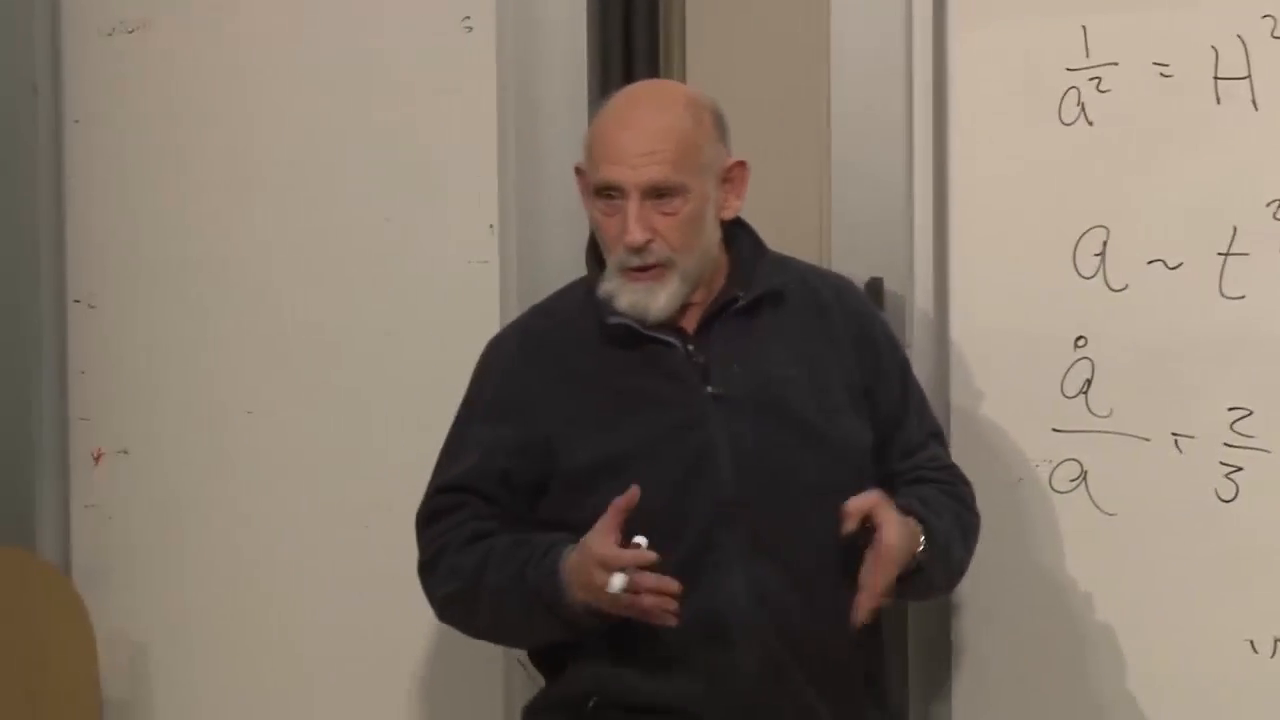
\includegraphics[width=0.72\textwidth]{lecture_06_figure_02.png}
\caption{Repaso de la pizarra de la era dominada por materia. En lo escrito se ven \(a\sim t^{2/3}\) y \(\dot a/a=2/(3t)\); el profesor oculta el resto de la pizarra, así que no se atribuye a la imagen ninguna ecuación que no sea visible.}
\label{fig:c06-age-board}
\lectureframe{00:24:41.615}
\end{figure}

\begin{classroomqa}
\audiencequestion{¿Qué unidades tiene la constante de Hubble y dónde aparece la velocidad de la luz?}
\lecturerresponse{Como \(H\) relaciona una velocidad con una distancia, sus unidades son de inverso del tiempo. Puede expresarse en segundos inversos, años inversos o en la unidad equivalente que usan los astrónomos: kilómetros por segundo por megapársec. La relación \(H\sim1/T\) no necesita ningún factor adicional de \(c\). Un factor de \(c\) aparece solo cuando el tiempo \(T\) se convierte en una longitud como \(cT\). \lecturetimestamp{00:22:50--00:24:25}}
\end{classroomqa}

El valor original de Hubble, \(H_0\), era demasiado grande por aproximadamente un orden de magnitud, por lo que la edad de Hubble correspondiente era demasiado corta: del orden de mil millones, en lugar de diez mil millones de años, según la comparación redondeada de la lección. Una calibración mejor corrigió el valor sin cambiar la lógica de que \(H_0^{-1}\) es una escala de tiempo cósmica.

La antigua inferencia sobre la curvatura se expresa ahora así:
\begin{equation}
\frac{1}{a_0^2}\sim H_0^2\sim\frac{1}{T^2}.
\end{equation}
En unidades \(c=1\), se pensaba, por tanto, que el radio de curvatura \(a_0\) era del orden de la edad \(T\); al restablecer las unidades habituales, era del orden de \(cT\). La lección enseguida deja claro que esto no describe el universo real. Es la conclusión a la que se llegaba varias décadas atrás, tras descartar los términos que entonces se creían despreciables.

\begin{classroomqa}
\audiencequestion{Si se suponía que la curvatura dominaba hoy, ¿por qué se usa la ley de dominación por materia \(a\propto t^{2/3}\)?}
\lecturerresponse{Porque la materia escala como \(a^{-3}\), mientras que la curvatura solo escala como \(a^{-2}\). Para valores menores de \(a\), domina la materia. La curvatura solo podía volverse importante en épocas tardías, así que la dominación por materia seguía describiendo la mayor parte de la historia transcurrida y mantenía \(H_0\) del orden de \(1/T\). Una solución mixta completa corregiría el factor numérico, pero no eliminaría el argumento sobre la escala temporal. \lecturetimestamp{00:49:20--00:50:17}}
\end{classroomqa}

\section{La materia oscura a partir de la dinámica galáctica}

Hay dos maneras operativas de contabilizar la materia. Una consiste en contar el material que emite o absorbe luz. La otra, en inferir la masa a partir de la gravedad. Oort encontró anomalías en la dinámica galáctica a comienzos de los años 1930, y Zwicky encontró una discrepancia análoga de masa en los cúmulos de galaxias. Las pruebas indicaban que la materia gravitante superaba a la materia luminosa. La materia ordinaria con carga eléctrica emite radiación y choca; al principio, el componente que faltaba se conocía por su acción gravitatoria.

\begin{classroomqa}
\audiencequestion{¿La materia luminosa incluye el gas difuso y los agujeros negros centrales?}
\lecturerresponse{El gas difuso se incluye en la medida en que su cantidad pueda inferirse a partir de su comportamiento electromagnético. Puede incluirse un agujero negro supermasivo central en el presupuesto de masa conocido, pero constituye solo una pequeña fracción de la masa total de una galaxia y está concentrado en el centro. No puede explicar una discrepancia que persiste mucho más allá del centro luminoso. \lecturetimestamp{00:29:50--00:31:14}}
\end{classroomqa}

Consideremos una estrella que se mueve aproximadamente en una órbita circular de radio \(r\). Si casi toda la masa \(M\) estuviera concentrada cerca del centro galáctico, la ley de Newton daría
\begin{equation}
\frac{GM}{r^2}=\frac{v^2}{r},
\end{equation}
y, por tanto,
\begin{equation}
v^2=\frac{GM}{r},
\qquad
v(r)\propto r^{-1/2}.
\label{eq:c06-kepler}
\end{equation}
Esta es la caída kepleriana que se espera fuera de una distribución de masa central.

\begin{figure}[htbp]
\centering
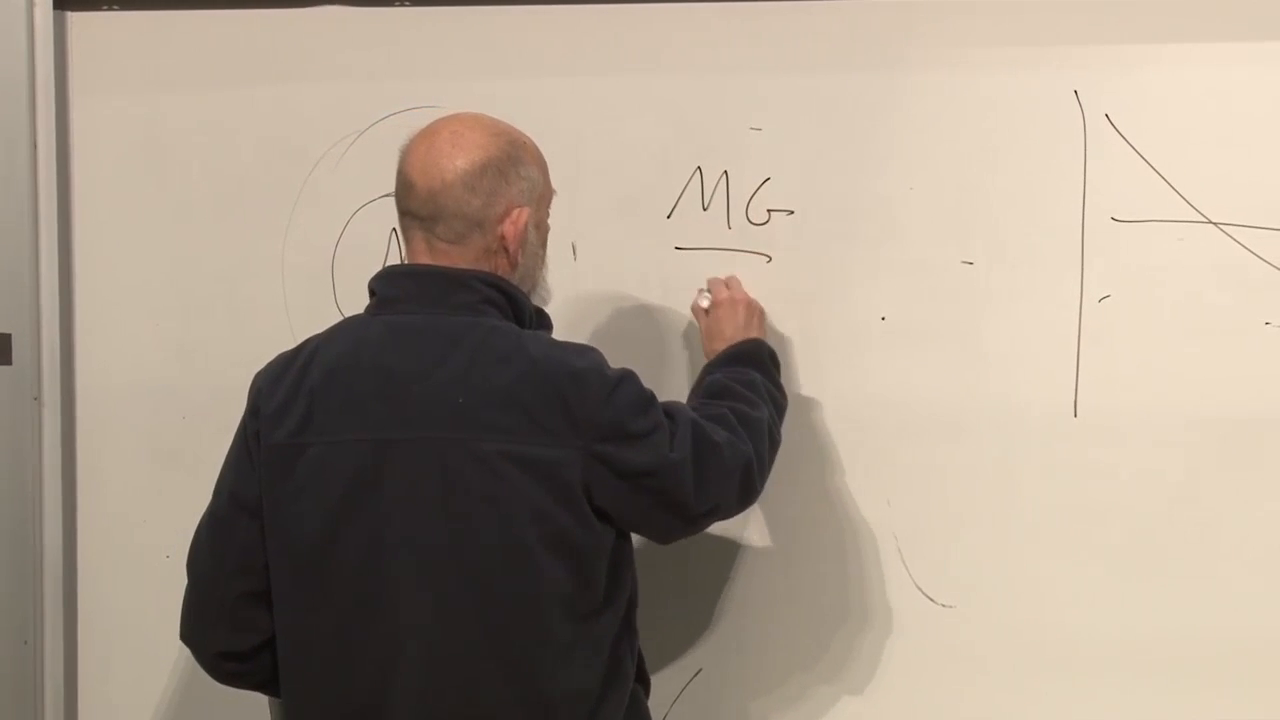
\includegraphics[width=0.78\textwidth]{lecture_06_figure_03.png}
\caption{La pizarra de las curvas de rotación, en la transición de una masa central a la masa encerrada \(M(r)\). Solo se ven \(MG\), la barra de fracción, el esquema de la órbita y partes de los esquemas de las curvas; la ecuación~\eqref{eq:c06-kepler} procede de la derivación oral.}
\label{fig:c06-rotation-board}
\lectureframe{00:34:53.642}
\end{figure}

\begin{figure}[htbp]
\centering
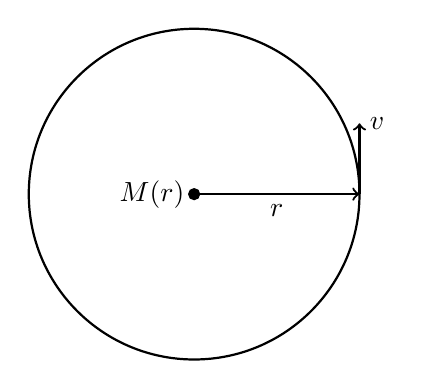
\begin{tikzpicture}[scale=1.0]
\filldraw (0,0) circle (2pt) node[left] {\(M(r)\)};
\draw[thick] (0,0) circle (2.1);
\draw[->,thick] (0,0)--(2.1,0) node[midway,below] {\(r\)};
\draw[->,thick] (2.1,0)--(2.1,0.9) node[right] {\(v\)};
\end{tikzpicture}
\caption{Construcción de la órbita circular utilizada para inferir la masa encerrada a partir de una velocidad de rotación medida.}
\label{fig:c06-orbit-redraw}
\end{figure}

Las curvas de rotación galáctica observadas no caen de esta manera; son aproximadamente planas en un intervalo radial considerable. Sustituyamos la masa central fija por la masa encerrada \(M(r)\):
\begin{equation}
\frac{G M(r)}{r^2}=\frac{v(r)^2}{r}.
\end{equation}
Si \(v(r)\) es casi constante, entonces
\begin{equation}
\boxed{M(r)\propto r.}
\label{eq:c06-enclosed-mass}
\end{equation}
Esto se refiere a la masa total dentro del radio \(r\), no a la densidad local. La masa gravitante sigue creciendo mucho más allá de la región donde se concentra la mayor parte de la luz estelar. Los movimientos perpendiculares a los discos galácticos indican, además, una distribución aproximadamente esférica: un halo oscuro, no un segundo disco delgado.

\begin{classroomqa}
\audiencequestion{¿Hay una teoría sencilla que explique por qué la curva de rotación es tan plana?}
\lecturerresponse{No dentro de este argumento. Las simulaciones de formación de galaxias pueden hacer que esos perfiles parezcan naturales, pero la lección no pretende ofrecer una derivación breve. La afirmación sólida es observacional: una velocidad \(v\) casi constante implica un crecimiento aproximadamente lineal de la masa encerrada. No debe confundirse la sencillez de esa relación con una explicación elemental de la formación galáctica. \lecturetimestamp{00:35:58--00:37:33}}
\end{classroomqa}

\begin{classroomqa}
\audiencequestion{¿Son los brazos espirales simples molinetes de materia producidos por la velocidad angular variable \(v/r\)?}
\lecturerresponse{No funciona ninguna imagen sencilla de un molinete. El patrón visible no tiene por qué girar junto con las estrellas individuales; entre las posibilidades están las descripciones mediante ondas de densidad o de formación estelar. La lección aprovecha esta incertidumbre para distinguir la inferencia sólida sobre el halo del problema más complejo de la estructura espiral. \lecturetimestamp{00:37:35--00:38:34; 00:47:03--00:47:47}}
\end{classroomqa}

La masa oscura inferida es varias veces mayor que la masa luminosa; en la lección se cita únicamente un factor aproximado, entre cinco y diez. El halo también se extiende más allá de la galaxia visible. Son órdenes de magnitud históricos deliberadamente aproximados, no proporciones universales precisas para todos los sistemas.

\section{Qué propiedades debe tener la materia oscura}

¿Por qué la materia ordinaria forma discos brillantes y compactos, mientras que la materia oscura permanece en un halo amplio? La materia luminosa puede perder energía mecánica mediante colisiones electromagnéticas y radiación. Al disipar energía, la gravedad puede atraerla hacia una configuración más densa. La materia oscura parece ser eléctricamente neutra y mucho menos interactuante. Sus partículas orbitan por el halo con pocas colisiones o emisiones de radiación, de modo que ni siquiera a lo largo de miles de millones de años pierden suficiente energía para asentarse en el disco luminoso. La radiación gravitatoria debida al movimiento galáctico es demasiado débil para ofrecer un mecanismo alternativo de enfriamiento.

\begin{classroomqa}
\audiencequestion{¿Que interactúe débilmente significa que la materia oscura obedece una ley de gravedad distinta?}
\lecturerresponse{No. Se supone que gravita de la manera habitual. En este contexto, «interacción débil» significa que las colisiones no gravitatorias y la radiación electromagnética están ausentes o muy suprimidas. Dos partículas oscuras siguen atrayéndose gravitatoriamente; esa atracción organiza un halo, pero no disipa eficazmente la energía orbital. \lecturetimestamp{00:42:36--00:43:35}}
\end{classroomqa}

\begin{classroomqa}
\audiencequestion{¿Qué observaciones indican que esto no es solo una peculiaridad de una curva de rotación galáctica?}
\lecturerresponse{Las pruebas aparecen a varias escalas: el movimiento de las estrellas dentro de las galaxias, el movimiento perpendicular a los planos galácticos, las interacciones entre galaxias y la dinámica de cúmulos galácticos enteros. Los ejemplos de Oort y Zwicky eran manifestaciones distintas del mismo problema de gravedad faltante. \lecturetimestamp{00:42:00--00:42:36}}
\end{classroomqa}

\begin{classroomqa}
\audiencequestion{¿Debería acumularse la materia oscura alrededor de los agujeros negros y los centros galácticos?}
\lecturerresponse{Su densidad sí aumenta hacia un centro gravitatorio, pero la secuencia histórica probablemente fue la inversa de la formación de un halo alrededor de un agujero negro preexistente. Los halos oscuros formaron pozos gravitatorios grandes; luego, la materia bariónica cayó en ellos y formó galaxias, estrellas y agujeros negros centrales. El agujero negro constituye una pequeña parte de la masa. Aun así, las búsquedas de productos de aniquilación apuntan al centro galáctico porque se espera que allí la densidad de materia oscura sea mayor. \lecturetimestamp{00:43:36--00:45:43}}
\end{classroomqa}

\begin{classroomqa}
\audiencequestion{¿La materia oscura es un gas, polvo, cúmulos compactos o partículas aisladas? ¿Podría haber materia oscura atrapada cerca del Sol?}
\lecturerresponse{Su naturaleza microscópica es desconocida, pero el polvo ordinario está ligado por fuerzas electromagnéticas, precisamente el tipo de interacción que parece faltarle a la materia oscura. Por eso, la imagen habitual es la de una población diluida de partículas individuales. Puede haber algunas concentradas gravitatoriamente cerca del Sol, pero su densidad es demasiado baja para competir con la gravedad solar o perturbar la dinámica planetaria. \lecturetimestamp{00:45:43--00:47:02; 00:58:41--00:59:29}}
\end{classroomqa}

El segundo requisito fundamental es que la materia oscura se agrupe. Una población caliente, con velocidades aleatorias relativistas, resiste la agregación gravitatoria; una población fría puede caer en pozos de potencial. Los neutrinos ordinarios, ligeros, se habrían comportado como materia oscura caliente y no aportan el componente galáctico principal requerido. En este contexto, \emph{fría} significa no relativista en el marco cosmológico local, no que tenga literalmente temperatura cero en el laboratorio.

\begin{classroomqa}
\audiencequestion{¿El requisito de agrupamiento en frío impone un intervalo de masas para la materia oscura?}
\lecturerresponse{Depende de la estadística cuántica y de la historia de producción. Fermiones muy ligeros no pueden ocupar todos un mismo estado lento y están sujetos a restricciones estrictas. Bosones muy ligeros pueden ocupar un estado coherente de condensación de Bose; los axiones son el ejemplo de la lección. Como alternativa, las partículas más pesadas que interactúan débilmente pueden estar frías sin condensarse. Por tanto, este argumento no proporciona un único límite de masa independiente del modelo. \lecturetimestamp{00:53:17--00:54:52; 00:56:42--00:58:05}}
\end{classroomqa}

\begin{classroomqa}
\audiencequestion{¿No deberían haber encontrado ya esas partículas los aceleradores?}
\lecturerresponse{Solo bajo hipótesis adicionales. Si las partículas tienen secciones eficaces de interacción débil aproximadamente típicas y masas dentro del alcance de los aceleradores, podría ser posible producirlas en colisionadores. La expectativa de la lección de obtener información pronto era explícitamente especulativa y propia de su época. Una partícula también podría ser demasiado pesada o interactuar demasiado débilmente para los experimentos disponibles. \lecturetimestamp{00:54:52--00:55:54}}
\end{classroomqa}

\begin{classroomqa}
\audiencequestion{¿Podría la materia oscura simplemente encontrarse en una dimensión extra invisible?}
\lecturerresponse{En esta discusión no se necesita tal mecanismo. La materia oscura ya se observa gravitatoriamente y podría estar formada simplemente por partículas inusuales que casi no interactúan con la materia ordinaria. Decir que una interacción es débil no equivale a situar las partículas fuera del espacio-tiempo observable. \lecturetimestamp{00:55:54--00:56:41}}
\end{classroomqa}

Modificar la gravedad en vez de añadir materia invisible es una alternativa lógica. La lección considera que, en aquel momento, ninguna modificación igual de sencilla explicaba las pruebas en todas las escalas pertinentes y, a la vez, conservaba las leyes del sistema solar que ya funcionaban. Por eso se prefiere la interpretación en términos de partículas, aunque su microfísica siga siendo desconocida.

\section{La materia oscura no cierra el antiguo balance}

La materia oscura aumenta varias veces la contribución de la materia, pero la antigua discrepancia entre la materia luminosa y \(H_0^2\) era del orden de veinticinco. Por tanto, reduce la diferencia sin hacer que se cumpla
\begin{equation}
\frac{C_m}{a_0^3}=H_0^2.
\end{equation}
Dentro del antiguo modelo sin \(\Lambda\), seguía siendo necesaria una contribución positiva al presupuesto de curvatura y, por tanto, \(k<0\). Ese modelo abierto no era lógicamente incoherente; el punto es que la materia oscura por sí sola no conducía a la respuesta moderna.

\begin{classroomqa}
\audiencequestion{¿Qué pensaban realmente los cosmólogos sobre la curvatura antes del ajuste moderno?}
\lecturerresponse{Las pruebas eran confusas, y la preferencia previa por un universo cerrado y acotado a veces entraba en conflicto con el balance de materia. Al combinar coherentemente las hipótesis antiguas, la inferencia natural era una curvatura negativa. Ese consenso histórico seguía siendo provisional porque ni la materia oscura ni la energía del vacío se habían incorporado de forma sólida como se hace hoy. \lecturetimestamp{00:50:17--00:51:50}}
\end{classroomqa}

Por tanto, debemos poner a prueba el modelo candidato, en vez de inferir que es verdadero a partir de una sola línea del balance. Un modelo consta de una elección de curvatura \(k\) y una historia de expansión \(a(t)\), o, de manera equivalente, de un conjunto de ecuaciones de estado de la materia y parámetros actuales a partir de los cuales se calcula \(a(t)\). El antiguo modelo candidato es el de materia más curvatura negativa, con radiación despreciable y sin constante cosmológica.

\section{Convertir la geometría en observables}

\subsection{Recuentos de fuentes y brillo en una geometría fija}

Por el momento, ignoremos la evolución cósmica. En un universo homogéneo, el número de fuentes en una capa comóvil es proporcional a su área:
\begin{equation}
dN\propto \xi(r)^2\,dr.
\label{eq:c06-shell-count}
\end{equation}
Por tanto,
\begin{equation}
dN\propto
\begin{cases}
\sin^2r\,dr, & k=+1,\\
r^2\,dr, & k=0,\\
\sinh^2r\,dr, & k=-1.
\end{cases}
\end{equation}
Para valores grandes de \(r\), el caso de curvatura negativa crece como \(\sinh^2r\sim e^{2r}\), mucho más deprisa que la ley plana \(r^2\). Así, la curvatura negativa predice un aumento anómalamente rápido del número de fuentes con la distancia.

La misma área determina el flujo recibido. En un espacio plano y estático, una fuente estándar da
\begin{equation}
F\propto\frac{1}{r^2}.
\end{equation}
En un espacio hiperbólico, la esfera sobre la que se propaga la radiación crece más deprisa, por lo que el flujo disminuye más rápidamente. A veces, la lección llama luminosidad a esta cantidad observada; aquí \(F\) denota el brillo o flujo, mientras que la luminosidad intrínseca corresponde a la fuente. Por tanto, los recuentos y el brillo, considerados conjuntamente, permiten distinguir las geometrías espaciales.

\subsection{Corrimiento al rojo y cono de luz pasado}

El universo real evoluciona y mirar hacia el exterior equivale a mirar hacia atrás en el tiempo. La luz emitida en \(t_{\rm em}\) se estira mientras el factor de escala crece de \(a(t_{\rm em})\) a \(a_0\):
\begin{equation}
1+z
=\frac{\lambda_{\rm obs}}{\lambda_{\rm em}}
=\frac{a_0}{a(t_{\rm em})}.
\label{eq:c06-redshift}
\end{equation}
De forma equivalente,
\begin{equation}
z=\frac{\lambda_{\rm obs}}{\lambda_{\rm em}}-1.
\end{equation}
Los distintos puntos de nuestro cono de luz pasado corresponden, al mismo tiempo, a radios comóviles distintos y a tiempos de emisión diferentes. La expansión cambia la longitud de onda; los corrimientos Doppler y gravitatorio son otros mecanismos físicos, pero aquí nos ocupa el efecto de la expansión cosmológica.

\begin{classroomqa}
\audiencequestion{¿Por qué la definición de \(z\) incluye el menos uno?}
\lecturerresponse{Es una convención histórica elegida para que una fuente sin corrimiento tenga \(z=0\). El factor de estiramiento directamente observable es \(1+z=\lambda_{\rm obs}/\lambda_{\rm em}\). \lecturetimestamp{01:10:11--01:10:45}}
\end{classroomqa}

Para la luz radial se tiene \(d\Omega_2=0\) y se cumple \(ds^2=0\). Por tanto, la ecuación~\eqref{eq:c06-frw} da
\begin{equation}
dt^2=a(t)^2dr^2.
\end{equation}
Para un rayo entrante, seguido hacia atrás desde nosotros,
\begin{equation}
dt=-a(t)\,dr,
\qquad
\frac{dr}{dt}=-\frac{1}{a(t)}.
\label{eq:c06-null-ray}
\end{equation}
El signo menos indica que, a lo largo del rayo, un radio comóvil mayor corresponde a un tiempo anterior. Una vez conocida \(a(t)\), esta ecuación determina \(r(t)\).

\subsection{Número por intervalo de corrimiento al rojo}

Un observador puede contar fuentes estándar en un intervalo de corrimiento al rojo entre \(z\) y \(z+dz\). Empecemos por la ecuación~\eqref{eq:c06-shell-count} y derivemos la ecuación~\eqref{eq:c06-redshift} a lo largo del rayo de luz pasado:
\begin{equation}
dz=-\frac{a_0}{a^2}\,da
=-\frac{a_0}{a^2}\dot a\,dt.
\end{equation}
Usando \(dt=-a\,dr\),
\begin{equation}
dz=\frac{a_0}{a}\dot a\,dr
=(1+z)\dot a\,dr.
\end{equation}
Por tanto,
\begin{equation}
dr=\frac{dz}{(1+z)\dot a},
\end{equation}
y, para una densidad fija de fuentes comóviles,
\begin{equation}
\boxed{
\frac{dN}{dz}
\propto
\frac{\xi(r)^2}{(1+z)\dot a}
}.
\label{eq:c06-dndz}
\end{equation}
La derivación en directo comprueba más de una vez los signos y los factores; las ecuaciones~\eqref{eq:c06-null-ray} y \eqref{eq:c06-redshift} fijan el resultado sin ambigüedad.

\begin{figure}[htbp]
\centering
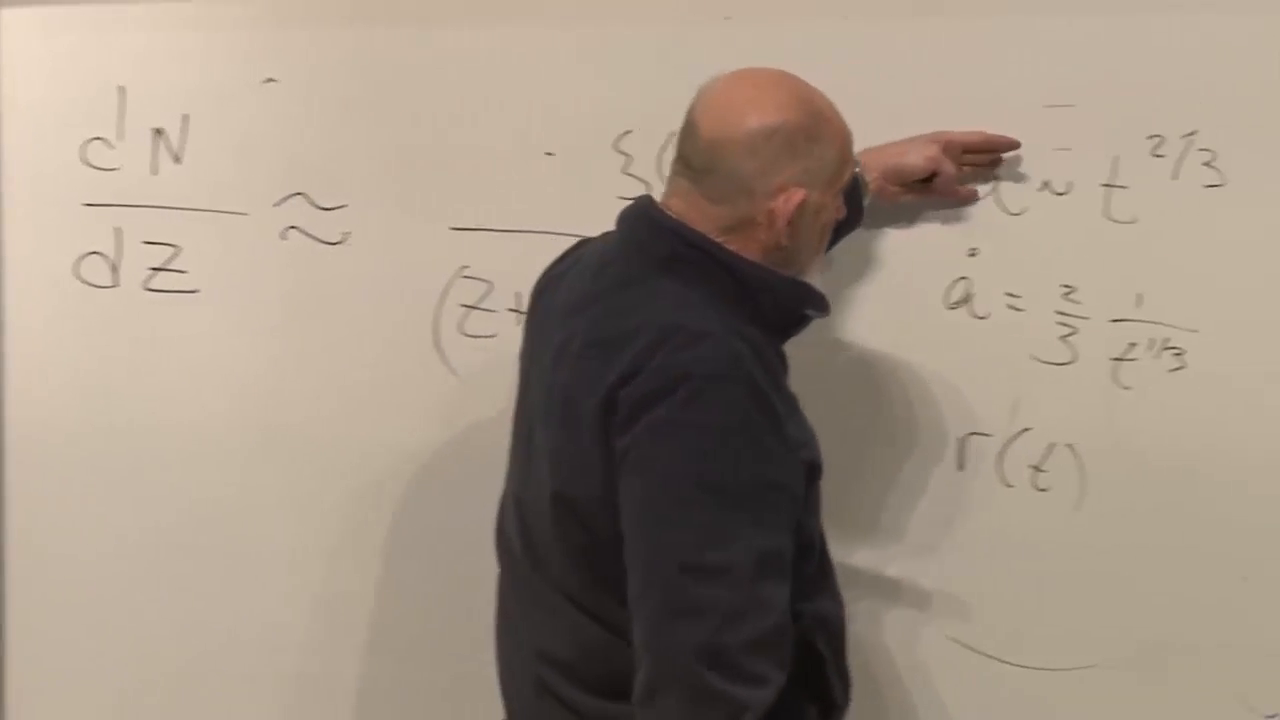
\includegraphics[width=0.84\textwidth]{lecture_06_figure_05.png}
\caption{Relación en la pizarra entre \(dN/dz\) y las funciones del modelo. Se ven el miembro izquierdo y \(a\sim t^{2/3}\), \(\dot a\) y \(r(t)\) en el derecho, pero el profesor oculta parte del denominador; la ecuación~\eqref{eq:c06-dndz} se estableció independientemente más arriba.}
\label{fig:c06-dndz-board}
\lectureframe{01:22:24.114}
\end{figure}

No hay nada más que calcular hasta elegir un modelo. Una \(a(t)\) especificada determina \(\dot a(t)\); la ecuación~\eqref{eq:c06-null-ray} determina \(r(t)\), y la ecuación~\eqref{eq:c06-redshift} permite expresar todas las cantidades en función de \(z\). Distintas ecuaciones de estado producen funciones \(dN/dz\) y \(F(z)\) distintas. Precisamente por eso las observaciones permiten discriminar entre modelos.

\section{De los parámetros tentativos al mejor ajuste}

El procedimiento es directo:
\begin{equation}
(\Omega_r,\Omega_m,\Omega_\Lambda,\Omega_k)
\longrightarrow
a(t)
\longrightarrow
\left\{F(z),\frac{dN}{dz}\right\}.
\label{eq:c06-fit-pipeline}
\end{equation}
Se eligen los parámetros actuales, se resuelve la ecuación de Friedmann, se propaga la luz radial, se calculan el brillo y los recuentos en función del corrimiento al rojo y se comparan las curvas con los datos. Una comparación fallida descarta ese conjunto de parámetros. En conjunto, los dos observables restringen tanto la historia de expansión como la geometría espacial.

\begin{figure}[htbp]
\centering
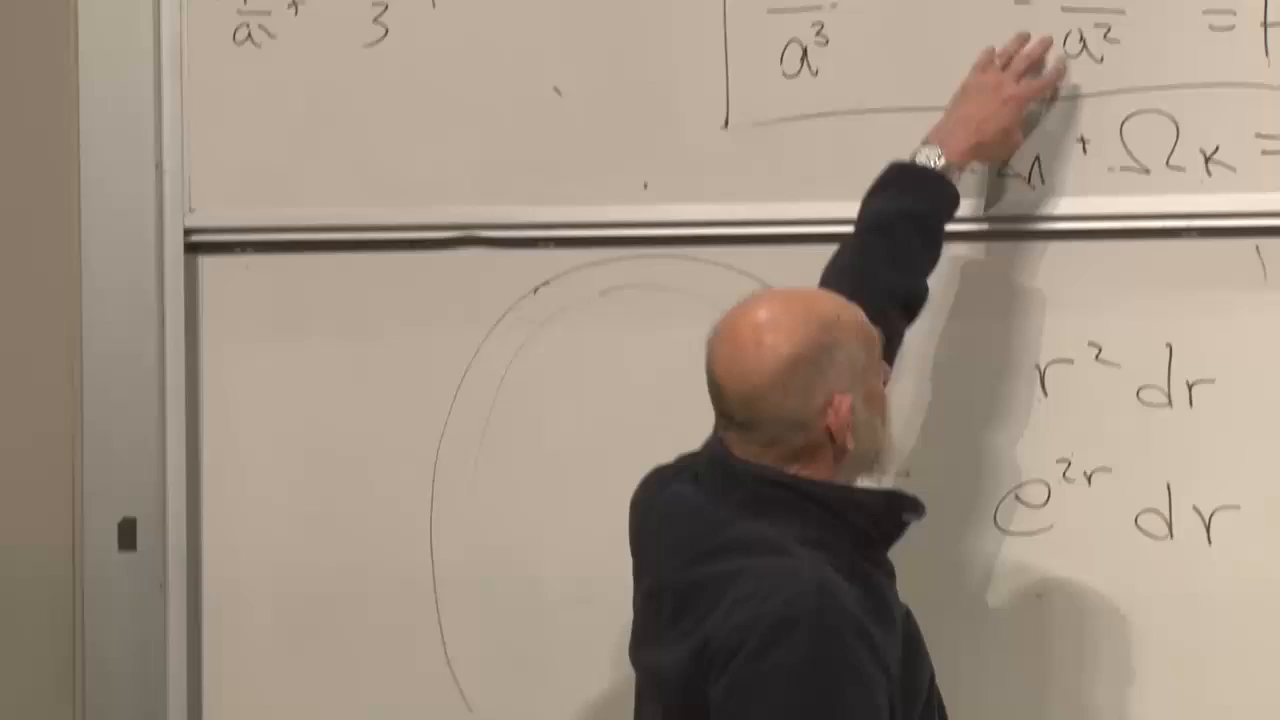
\includegraphics[width=0.84\textwidth]{lecture_06_figure_06.png}
\caption{El antiguo modelo de materia más curvatura en la parte superior de la pizarra y los factores de las capas plana e hiperbólica \(r^2dr\) y \(e^{2r}dr\) en la parte inferior. Hay partes de la ecuación de Friedmann cubiertas, así que la imagen sirve como apoyo, no como fuente de una ecuación.}
\label{fig:c06-old-model-board}
\lectureframe{01:24:27.863}
\end{figure}

El modelo antiguo,
\begin{equation}
H^2=\frac{C_m}{a^3}-\frac{k}{a^2},
\qquad k=-1,
\end{equation}
no concuerda ni con la relación entre brillo y corrimiento al rojo ni con la prueba de recuento de fuentes. Las supernovas proporcionan las candelas estándar más útiles en el intervalo de corrimientos al rojo pertinente. El conjunto de parámetros que da un ajuste satisfactorio en la lección es
\begin{equation}
\boxed{
\Omega_r\simeq0,\qquad
\Omega_m\simeq0.3,\qquad
\Omega_\Lambda\simeq0.7,\qquad
\Omega_k\simeq0
}.
\label{eq:c06-best-fit}
\end{equation}
Aquí, la materia incluye tanto la materia luminosa como la oscura. Estos valores corresponden al ajuste de la época de la lección; la enseñanza duradera es el método de ajuste y la necesidad de un componente dominante que no se diluya, no el último decimal impreso.

\subsection{Preguntas sobre qué se mide y qué se ajusta}

\begin{classroomqa}
\audiencequestion{¿Se había supuesto ya \(\Lambda\) al hablar del antiguo modelo de universo abierto?}
\lecturerresponse{No. La primera parte reconstruyó deliberadamente el modelo antiguo con \(\Lambda=0\). Los valores de la ecuación~\eqref{eq:c06-best-fit} describen el ajuste moderno posterior. El antiguo modelo candidato no se modificó sin decirlo: se puso a prueba frente a \(F(z)\) y \(dN/dz\) y no funcionó. \lecturetimestamp{01:26:45--01:27:07}}
\end{classroomqa}

\begin{classroomqa}
\audiencequestion{¿Cómo se obtiene \(\Omega_\Lambda\) si la energía del vacío no se mide directamente como la materia local?}
\lecturerresponse{Se empieza con conjuntos tentativos de parámetros. Cada conjunto define una solución de Friedmann y, por tanto, las funciones predichas \(F(z)\) y \(dN/dz\). Se comparan esas predicciones con las observaciones, se descartan los ajustes deficientes y se conserva la región del espacio de parámetros que ofrece el mejor ajuste. El valor \(0.7\) se infiere del ajuste; no es la lectura directa de un medidor de energía del vacío. \lecturetimestamp{01:27:08--01:29:59; 01:31:57--01:33:40}}
\end{classroomqa}

\begin{classroomqa}
\audiencequestion{¿De dónde procede la escala actual \(a_0\)?}
\lecturerresponse{La normalización de \(a\) es en parte convencional, pero un modelo completo ligado a \(H_0\) proporciona la escala física de curvatura actual cuando \(k\ne0\). Una vez que el modelo ajusta los observables de corrimiento al rojo, su función \(a(t)\) identifica el instante presente y la escala correspondiente. \lecturetimestamp{01:29:59--01:30:42}}
\end{classroomqa}

\begin{classroomqa}
\audiencequestion{¿Mirar miles de millones de años hacia el pasado distorsiona un ajuste basado en los parámetros actuales?}
\lecturerresponse{La mirada retrospectiva no es una distorsión, sino la señal. Los parámetros actuales se introducen en la ecuación de Friedmann, que los hace evolucionar hasta formar un \(a(t)\) completo. El cono de luz predicho ya incorpora que la materia tenía mayor importancia cuando \(a\) era menor y que, al retroceder lo suficiente, domina la radiación. Un modelo que ignorara esta evolución no concordaría con los datos. \lecturetimestamp{01:30:43--01:31:55}}
\end{classroomqa}

\begin{classroomqa}
\audiencequestion{¿Qué magnitudes actuales se miden de forma relativamente directa?}
\lecturerresponse{La densidad de radiación se mide y hoy es despreciable. La tasa de Hubble se mide a partir de la relación entre distancia y corrimiento al rojo. La densidad total de materia se infiere gravitacionalmente, incluida la materia luminosa y la oscura, y se divide por la escala crítica \(3H_0^2/(8\pi G)\) para obtener \(\Omega_m\). La libertad restante en épocas tardías reside principalmente en la energía del vacío y la curvatura. \lecturetimestamp{01:33:40--01:35:32}}
\end{classroomqa}

\begin{classroomqa}
\audiencequestion{Si se desconocen tanto \(\Omega_\Lambda\) como \(\Omega_k\), ¿por qué queda un solo parámetro de prueba independiente para épocas tardías una vez fijado \(\Omega_m\)?}
\lecturerresponse{Porque la ecuación~\eqref{eq:c06-sum-rule} impone una restricción. Si \(\Omega_r\) es despreciable y \(\Omega_m\) está medido, elegir un valor de prueba para \(\Omega_\Lambda\) determina el \(\Omega_k=1-\Omega_m-\Omega_\Lambda\) restante. También se puede parametrizar la misma familia unidimensional mediante la curvatura. Por ejemplo, \(\Omega_\Lambda=0.4\) y \(\Omega_k=0.3\) constituye una elección de prueba válida cuando \(\Omega_m=0.3\); se descarta únicamente porque sus curvas predichas ajustan mal los datos, no porque la regla de suma lo prohíba. \lecturetimestamp{01:35:33--01:39:09}}
\end{classroomqa}

\begin{classroomqa}
\audiencequestion{¿Cómo puede \(k\) tener solo los valores \(+1,0,-1\) mientras \(\Omega_k\) varía continuamente? ¿Son correctas las dimensiones?}
\lecturerresponse{El valor discreto de \(k\) solo registra el signo y la geometría normalizada. El radio de curvatura continuo está dado por \(a_0\), de modo que \(-k/(a_0^2H_0^2)\) puede tomar un continuo de valores. En unidades \(c=1\), la longitud inversa y el tiempo inverso tienen las mismas dimensiones; al restituir las unidades convencionales aparecen las potencias necesarias de \(c\). \lecturetimestamp{01:39:10--01:40:07}}
\end{classroomqa}

\begin{classroomqa}
\audiencequestion{¿El método de conteo supone homogeneidad e isotropía, aunque las poblaciones de galaxias evolucionen?}
\lecturerresponse{Supone homogeneidad e isotropía espacial en hipersuperficies suficientemente grandes, y estas simetrías pueden ponerse a prueba comparando distintas direcciones al mismo corrimiento al rojo. La evolución de las fuentes es una cuestión aparte: las poblaciones de distintas épocas no tienen por qué ser idénticas, así que los análisis prácticos modelan los efectos de selección y la evolución, en vez de fingir que la densidad numérica permanece fija para siempre. La derivación sencilla aísla el factor geométrico antes de incorporar esos refinamientos. \lecturetimestamp{01:40:08--01:41:08}}
\end{classroomqa}

\section{Las fracciones de densidad evolucionan}

La ecuación~\eqref{eq:c06-budget} se cumple en todo instante, pero los \(\Omega\) de la ecuación~\eqref{eq:c06-omegas} se definieron para el instante presente. Sus análogos dependientes del tiempo cambian porque los cuatro términos tienen distintas potencias de \(a\). En el pasado remoto,
\begin{equation}
\Omega_r(t)\longrightarrow1.
\end{equation}
A medida que la radiación se diluye más deprisa, la materia va acercándose al dominio. Más adelante, la materia también se diluye, mientras que \(\Lambda\) permanece constante; por tanto, en el futuro remoto,
\begin{equation}
\Omega_\Lambda(t)\longrightarrow1.
\end{equation}
La fracción de materia empieza siendo pequeña, se acerca a la unidad durante la era dominada por la materia y vuelve a disminuir cuando la energía del vacío pasa a dominar. Si la curvatura no es nula, también acaba siendo superada por una constante positiva \(\Lambda\).

\begin{classroomqa}
\audiencequestion{¿Una fracción de curvatura actual pequeña significa que el universo se vuelve más plano al expandirse?}
\lecturerresponse{Su escala física de curvatura crece con \(a\) y, respecto de una constante cosmológica positiva, la contribución de la curvatura \(a^{-2}\) pierde cada vez más importancia. Ese es el sentido de la expresión \emph{grande es plano}. Esto no cambia la etiqueta discreta de topología \(k\); significa que disminuyen la curvatura local y la importancia dinámica fraccionaria de la curvatura. \lecturetimestamp{01:47:13--01:47:42}}
\end{classroomqa}

\begin{classroomqa}
\audiencequestion{¿El modelo ajustado mostró residuos sistemáticos sin explicación, y cuán precisa era la afirmación?}
\lecturerresponse{La conferencia no señala ningún fallo sistemático conocido del marco teórico a ese nivel y lo describe como cosmología de precisión, con una exactitud del orden del uno por ciento, no de una décima ni de una centésima de punto porcentual. Esa afirmación es histórica y no debe convertirse en una barra de error actual y atemporal. \lecturetimestamp{01:45:40--01:46:19}}
\end{classroomqa}

\begin{classroomqa}
\audiencequestion{¿Se puede poner a prueba la curvatura espacial mediante triangulación directa, en vez de basarse solo en el brillo de las supernovas y los conteos?}
\lecturerresponse{Sí. El patrón angular de la radiación cósmica de fondo proporciona una escala física estándar y, por tanto, un gran triángulo cósmico. Los datos de supernovas por sí solos no bastaban para sustentar la afirmación de la conferencia sobre la curvatura con una precisión del uno por ciento; al combinarlos con la geometría de la radiación de fondo, la prueba se volvió más precisa. Este es el tema de la siguiente conferencia. \lecturetimestamp{01:46:19--01:47:12}}
\end{classroomqa}

\section{Ideas clave}

La lección central no es un catálogo de cuatro números, sino un método. Un conjunto de parámetros cosmológicos determina \(a(t)\); la métrica predice entonces la propagación de la luz, el brillo de las fuentes y su conteo. La concordancia pone a prueba tanto los parámetros elegidos como el marco de Friedmann que los relaciona. No hay motivo para que un conjunto arbitrario ajuste los datos.

El antiguo modelo de materia luminosa y curvatura negativa fracasó. La materia oscura corrigió el inventario de materia gravitante, pero por sí sola no cerró el antiguo balance de Friedmann. El ajuste satisfactorio de la época de la conferencia requería aproximadamente
\begin{equation}
\Omega_m\simeq0.3,
\qquad
\Omega_\Lambda\simeq0.7,
\qquad
\Omega_k\simeq0,
\end{equation}
y su precisión en la curvatura dependía de manera importante de la radiación cósmica de fondo. El modelo resulta creíble porque varias observaciones independientes se interpretan mediante una misma teoría dinámica y convergen en la misma región del espacio de parámetros.
